\documentclass[11pt,a4paper]{article}

% ============================================
% PACKAGES
% ============================================
\usepackage[utf8]{inputenc}
\usepackage[T1]{fontenc}
\usepackage{lmodern}
\usepackage[margin=2.5cm]{geometry}
\usepackage{amsmath,amssymb,amsthm}
\usepackage{graphicx}
\usepackage{booktabs}
\usepackage{array}
\usepackage{enumitem}
\usepackage{xcolor}
\usepackage{hyperref}
\usepackage{cleveref}
\usepackage{tikz}
\usetikzlibrary{arrows.meta,positioning,shapes,calc,decorations.pathreplacing}
\usepackage{natbib}
\usepackage{caption}
\usepackage{float}

% ============================================
% CUSTOM COLORS (consistent with Paper 1)
% ============================================
\definecolor{exitcolor}{RGB}{220,53,69}
\definecolor{codecolor}{RGB}{40,167,69}
\definecolor{auditcolor}{RGB}{0,123,255}
\definecolor{governcolor}{RGB}{255,193,7}
\definecolor{forkcolor}{RGB}{111,66,193}

% ============================================
% THEOREM ENVIRONMENTS
% ============================================
\theoremstyle{definition}
\newtheorem{definition}{Definition}[section]
\newtheorem{proposition}{Proposition}[section]
\newtheorem{principle}{Principle}[section]
\newtheorem{claim}{Claim}[section]

% ============================================
% CUSTOM COMMANDS
% ============================================
\newcommand{\papertitle}{Corrigibility for Learned Systems: Extending Structural Accountability to AI}

% ============================================
% METADATA
% ============================================
\title{\papertitle}
\author{Working Draft}
\date{February 2026}

% ============================================
% KEYWORDS ENVIRONMENT
% ============================================
\newenvironment{keywords}{\paragraph{Keywords:}}{}

% ============================================
% DOCUMENT
% ============================================
\begin{document}

\maketitle

\begin{abstract}
This paper extends the corrigibility framework for Digital Public Infrastructure (DPI) to learned systems---AI models whose behavior is determined by training data rather than explicit code. While the companion paper establishes five structural tests (EXIT, CODE, AUDIT, GOVERN, FORK) for infrastructure accountability, learned systems present unique challenges: stochastic outputs, opaque training pipelines, compute-gated reproduction, and temporal variety gaps. We demonstrate that the five tests remain invariant for AI systems; only the verification methods change. The paper introduces three contributions: (1) the \textbf{LWD-R disclosure requirement} extending CODE to training pipelines, (2) the \textbf{Temporal Variety Gap} explaining why AI corrigibility requires ongoing governance rather than deployment-time verification, and (3) \textbf{Compute Capture} as a resource barrier to FORK that transforms ``open weights'' into performative transparency. Analysis of agentic scaling reveals that incorrigible infrastructure becomes structurally incompatible with AI automation, producing Governance Denial of Service (GDoS). The framework provides falsifiable tests for AI infrastructure accountability, distinguishing structural corrigibility from operator-focused ``AI alignment.''
\end{abstract}

\begin{keywords}
AI Governance, Corrigibility, Learned Systems, Compute Capture, Agentic Economy, LWD-R, Open Source AI
\end{keywords}

\section{Introduction}
\label{sec:intro}

The companion paper \citep{paper1} establishes a corrigibility framework for Digital Public Infrastructure, deriving five structural tests from cybernetics, commons governance, and free software:

\begin{itemize}[noitemsep]
    \item \textbf{EXIT}: Reversibility of participation
    \item \textbf{CODE}: Inspectability of logic
    \item \textbf{AUDIT}: Independent verification
    \item \textbf{GOVERN}: Binding constraint
    \item \textbf{FORK}: Capacity to reproduce
\end{itemize}

This paper stress-tests the framework against learned systems---infrastructure where behavior is determined by parameters learned from data (AI/ML) rather than explicit code logic. If the five tests are truly fundamental, they must apply not only to deterministic infrastructure but also to stochastic systems where traditional verification assumptions collapse.

\paragraph{The Challenge.} Learned systems dismantle the assumption that source code is the sole arbiter of behavior. In AI, identical inputs may yield stochastic outputs; behavior is defined by training data; and opacity is often inherent rather than contrived. Yet the collapse of deterministic transparency does not invalidate corrigibility's structural necessity. As systems become less intelligible, external correction becomes \textit{more} critical.

\paragraph{Thesis.} The five corrigibility tests remain invariant for learned systems. What changes is the verification method and the resource barriers to compliance.

\paragraph{Scope.} This paper addresses AI systems deployed as infrastructure---models that determine citizen outcomes at scale. It does not address consumer AI products where exit is trivial, nor research systems without deployment impact. The focus is on AI that functions as DPI: identity verification models, welfare eligibility systems, public-facing chatbots with administrative authority, and autonomous agents operating within mandatory infrastructure.

\paragraph{Paper Structure.} Section~\ref{sec:invariance} establishes that the five tests remain invariant. Section~\ref{sec:code-ai} extends the CODE test via the LWD-R disclosure requirement. Section~\ref{sec:temporal} introduces the Temporal Variety Gap. Section~\ref{sec:fork-ai} analyzes resource barriers to FORK, including compute capture. Section~\ref{sec:agentic} examines agentic scaling and Governance Denial of Service. Section~\ref{sec:workflow} addresses workflow sovereignty and the Rule of Workflow. Section~\ref{sec:architecture} provides architecture-specific risk analysis. Section~\ref{sec:discussion} discusses implications and limitations.

%% ============================================
%% SECTION 2: INVARIANCE
%% ============================================

\section{The Invariance of the Standard}
\label{sec:invariance}

\begin{proposition}
The five corrigibility tests remain invariant for learned systems. What changes is the verification method.
\end{proposition}

The structural requirement for corrigibility derives from Ashby's Law of Requisite Variety: a controller must have at least as many response states as the system it governs \citep{ashby1956}. This requirement is independent of whether the controlled system is deterministic or stochastic. An AI model that affects citizen outcomes at population scale generates the same variety of potential harms as deterministic infrastructure; therefore, the governance apparatus must possess equivalent corrective variety.

The table below illustrates how the mechanical verification of each test adapts to the probabilistic nature of AI without softening the structural requirement.

\begin{table}[htbp]
\centering
\begin{tabular}{@{}lll@{}}
\toprule
\textbf{Test} & \textbf{Deterministic Verification} & \textbf{Learned System Verification} \\
\midrule
EXIT & Can refuse the system & Disclosure + non-AI alternative \\
CODE & Source code determines behavior & Layered transparency across training pipeline \\
AUDIT & Inspect logic and outputs & Statistical bounds + continuous monitoring \\
GOVERN & Maintainer and RFC process & Governance over objectives and value tradeoffs \\
FORK & Copy code and deploy & Resource forkability (compute + data) \\
\bottomrule
\end{tabular}
\caption{Verification methods for deterministic vs. learned systems}
\label{tab:verification}
\end{table}

\paragraph{Key Insight.} The shift from deterministic to learned systems does not weaken the tests; it \textit{strengthens} the case for structural corrigibility. When behavior becomes less predictable, the capacity for external correction becomes more essential. A deterministic system that fails silently can be debugged; a learned system that fails silently accumulates error without detection.

%% ============================================
%% SECTION 3: CODE FOR AI (LWD-R)
%% ============================================

\section{What Is ``Source'' in a Learned System?}
\label{sec:code-ai}

A central challenge in complying with the \textbf{CODE} test is redefining the object of inspection. In a learned system, behavior is distributed across a lineage of distinct artifacts. The inference code is merely the execution engine; the actual behavioral logic is encoded in the weights, which are in turn downstream of the training corpus, filtering decisions, and RLHF preferences.

\begin{principle}[Source Distribution]
Publishing inference code alone does not satisfy the CODE test. It allows an auditor to run the machine, but not to understand why it produces specific outputs.
\end{principle}

To bridge this gap, compliance requires structured disclosure across the training pipeline, such as \textbf{Data Sheets for Datasets} \citep{gebru2021} and \textbf{Model Cards} \citep{mitchell2019}. These artifacts function as the ``source code'' for structural evaluation; withholding them renders the system a black box.

\subsection{The LWD-R Disclosure Requirement}

For world models and agentic systems, the traditional transparency requirements (code, weights, data) are necessary but insufficient. We extend the disclosure requirement to the \textbf{LWD-R Triad}:

\begin{definition}[LWD-R]
\label{def:lwdr}
A learned system satisfies LWD-R disclosure if the following artifacts are publicly available:
\begin{itemize}[noitemsep]
    \item \textbf{L (Logic)}: Model architecture and inference code
    \item \textbf{W (Weights)}: Trained parameters
    \item \textbf{D (Data)}: Training corpus with provenance (Data Sheets)
    \item \textbf{R (Representation Schema)}: The ontological categories the model uses to parse reality
\end{itemize}
\end{definition}

The fourth component, \textbf{R}, is critical for world models that encode a de facto administrative ontology. When an AI system classifies citizens, transactions, or risks, it instantiates categories that become infrastructural facts. Failure to disclose \textbf{R} renders the model's worldview non-inspectable.

\subsection{Ontological Opacity and Representation Capture Risk}
\label{subsec:rcr}

We define \textbf{Representation Capture Risk (RCR)} as the condition where a society becomes dependent on a model's categorical schema without structural means to contest or modify those categories.

\begin{definition}[Representation Capture Risk]
Let $\Delta O$ represent the \textbf{ontological contestability} of a system, defined as the degree to which affected parties can challenge, modify, or replace the representation schema. RCR occurs when:
\begin{equation}
\Delta O \to 0
\end{equation}
\end{definition}

Under RCR, the model's internal categories become non-contestable administrative facts. A welfare eligibility model that classifies applicants into risk tiers, or a world model that parses geopolitical actors into threat categories, exercises definitional power over reality. When $\Delta O = 0$, the system fails CODE not because the weights are hidden, but because the \textit{meaning structure} is opaque.

\paragraph{Extension to CODE.} This extends the CODE test for world models: compliance requires not merely weight publication but \textbf{representation schema disclosure}---machine-readable specifications of the ontological categories the model employs, with documented justification for category boundaries.

%% ============================================
%% SECTION 4: TEMPORAL VARIETY GAP
%% ============================================

\section{The Temporal Variety Gap}
\label{sec:temporal}

A central theoretical contribution of this framework is the identification of the \textbf{Temporal Variety Gap}: a fundamental challenge that distinguishes learned systems from traditional infrastructure and explains why AI corrigibility requires ongoing governance, not merely deployment-time verification.

Unlike traditional software, which remains static until explicitly patched, learned systems possess a distinct vulnerability related to time. The variety of the controller ($V_c$) is frozen at the moment of training parameterization ($\theta$), while the variety of the world it operates upon ($V_d$) continues to expand.

\begin{equation}
\Delta(t) = V(\text{disturbance}; t) - V(\text{controller}; \theta)
\label{eq:variety-gap}
\end{equation}

Without mechanisms for retraining or fine-tuning accessible to the community, the variety gap $\Delta(t)$ widens over time. Thus, AI corrigibility is not a deployment property, but a \textit{persistence condition}.

\begin{figure}[htbp]
\centering
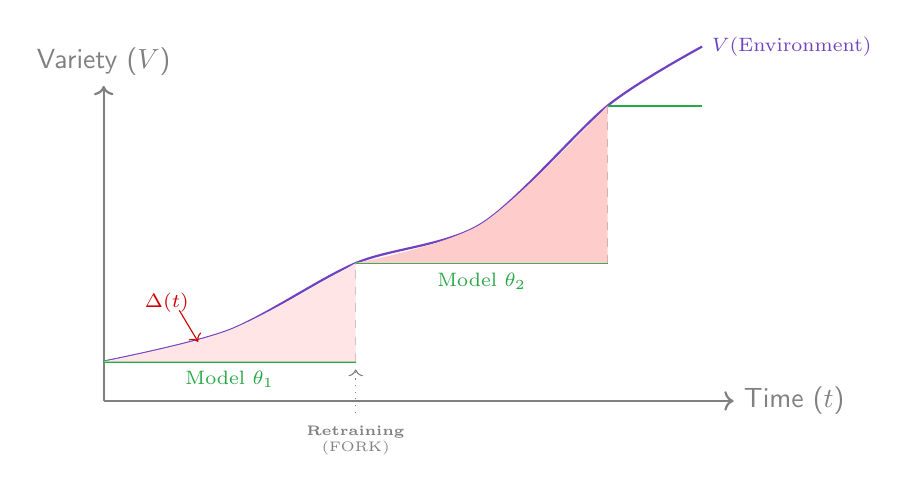
\begin{tikzpicture}[x=0.8cm, y=0.5cm, font=\sffamily]

    % Axes
    \draw[->, thick, gray] (0,0) -- (10,0) node[right] {Time ($t$)};
    \draw[->, thick, gray] (0,0) -- (0,8) node[above] {Variety ($V$)};

    % Real World Complexity (The Disturbance) - Curving up
    \draw[thick, forkcolor, smooth] plot coordinates {(0,1) (2,1.8) (4,3.5) (6,4.5) (8,7.5) (9.5, 9)};
    \node[forkcolor, anchor=west, font=\scriptsize] at (9.5, 9) {$V(\text{Environment})$};

    % AI Model State (The Controller) - Step Function
    \draw[thick, codecolor] (0,1) -- (4,1);
    \draw[dashed, gray] (4,1) -- (4,3.5);
    \draw[thick, codecolor] (4,3.5) -- (8,3.5);
    \draw[dashed, gray] (8,3.5) -- (8,7.5);
    \draw[thick, codecolor] (8,7.5) -- (9.5,7.5);

    % Labels for Model
    \node[codecolor, anchor=north, font=\scriptsize] at (2,1) {Model $\theta_1$};
    \node[codecolor, anchor=north, font=\scriptsize] at (6,3.5) {Model $\theta_2$};

    % The Gap (Error)
    \fill[red!10] (0,1) -- (4,1) -- (4,3.5) -- plot[smooth] coordinates {(4,3.5) (2,1.8) (0,1)} -- cycle;
    \fill[red!20] (4,3.5) -- (8,3.5) -- (8,7.5) -- plot[smooth] coordinates {(8,7.5) (6,4.5) (4,3.5)} -- cycle;

    % Annotations
    \node[anchor=west, text=red!80!black, font=\scriptsize] at (0.5, 2.5) {$\Delta(t)$};
    \draw[->, red!80!black] (1.2, 2.3) -- (1.5, 1.5);

    \node[align=center, font=\tiny, gray] at (4, -1) {\textbf{Retraining}\\(FORK)};
    \draw[->, gray, dotted] (4, -0.3) -- (4, 0.8);

\end{tikzpicture}
\caption{\textbf{The Temporal Variety Gap.} Environmental variety $V(e)$ evolves continuously (curve). A fixed model $\theta$ (stepped line) diverges from reality. The shaded area represents accumulated error. Only \textbf{FORK} rights allow the gap to be closed via retraining.}
\label{fig:variety_gap}
\end{figure}

\begin{claim}
A learned system that passes all five corrigibility tests at deployment may fail them over time if the community lacks the resources to retrain. Corrigibility for AI is a dynamic property, not a static certification.
\end{claim}

%% ============================================
%% SECTION 5: FORK AND COMPUTE CAPTURE
%% ============================================

\section{Resource Barriers to Forkability}
\label{sec:fork-ai}

The right to \textbf{FORK} a learned system is constrained by physical resources rather than just copyright. In traditional software, the cost to fork is the cost of storage; in AI, the cost to fork is the cost of compute.

\begin{table}[htbp]
\centering
\begin{tabular}{@{}lll@{}}
\toprule
\textbf{Layer} & \textbf{Cost} & \textbf{Barrier} \\
\midrule
Inference code & Minimal & None \\
Running open weights & Low & Minor \\
Fine-tuning & Moderate & Economic \\
Retraining from scratch & Very high & Structural \\
\bottomrule
\end{tabular}
\caption{Resource barriers to forking learned systems}
\label{tab:fork-barriers}
\end{table}

\begin{claim}
Legal permission to fork without access to compute or data is meaningless. This is an infrastructure question, not a licensing question.
\end{claim}

\subsection{The Compute Capture Problem}
\label{subsec:compute-capture}

\begin{principle}[Compute Capture]
Training forkability is functionally impossible when the compute cost to retrain a model exceeds the compute accessible to plausible non-operator actors by more than a policy-determined multiplier. Releasing weights while hoarding compute is \textbf{inference forkability without training forkability}.
\end{principle}

If a company releases weights but training cost exceeds 100$\times$ global academic compute capacity, training forkability is zero.

\paragraph{Formal Definition.} Let $C_{\text{train}}$ be the compute cost required to retrain a model, and $C_{\text{accessible}}$ be the compute accessible to plausible non-operator actors (academic clusters, government research consortiums, distributed compute pools). Training forkability is functionally impossible when:
\begin{equation}
C_{\text{train}} > \kappa \cdot C_{\text{accessible}}
\label{eq:compute-capture}
\end{equation}
where $\kappa$ is an accessibility multiplier (policy constant, typically $1 \leq \kappa \leq 2$).

The formal FORK determination for training becomes:
\begin{equation}
\text{FORK}_{\text{training}} = \mathbf{1}[C_{\text{train}} \leq \kappa \cdot C_{\text{accessible}}] \land \mathbf{1}[\text{data\_manifest\_available}]
\label{eq:fork-training}
\end{equation}
where $\mathbf{1}[\cdot]$ is the indicator function.

\subsection{Compute as Governance Infrastructure}

This analysis implies that \textbf{compute is itself DPI}. Legal forkability is insufficient absent practical compute accessibility. Architectural responses include:
\begin{enumerate}[noitemsep]
    \item \textbf{Public Compute Nodes}: State-sponsored clusters with multi-stakeholder governance
    \item \textbf{Mandatory Cost Disclosure}: FLOP estimates and data manifests
    \item \textbf{Federated Training Pools}: Distributed training across independent nodes
    \item \textbf{Compute Vouchers}: Grants for reproduction attempts
\end{enumerate}

\subsection{Minimum Evidence for Learned System Forkability}
\label{subsec:fork-evidence}

To prevent ``FORK fails'' from becoming a rhetorical claim rather than a verifiable determination, learned systems must satisfy specific evidentiary requirements:

\begin{table}[htbp]
\centering
\small
\caption{Evidence requirements for FORK in learned systems}
\label{tab:ai-fork-evidence}
\begin{tabular}{@{}llp{5.5cm}@{}}
\toprule
\textbf{Artifact} & \textbf{Status} & \textbf{Verification} \\
\midrule
Inference code & Required & Open source license; build reproducibility \\
Model weights & Required & Public download; hash verification \\
Training data manifest & Required & Data Sheets \citep{gebru2021} with provenance \\
Training checkpoint & Recommended & Enables fine-tuning without full retrain \\
Training code & Required & Includes preprocessing, hyperparameters \\
Compute cost estimate & Required & FLOP estimate or cloud cost documentation \\
Successful reproduction & Decisive & Third-party retrain within 10\% of benchmark \\
\bottomrule
\end{tabular}
\end{table}

\paragraph{Forkability Determination.} A learned system passes FORK if:
\begin{enumerate}[noitemsep]
    \item All ``Required'' artifacts are publicly available under permissive terms
    \item The compute cost estimate demonstrates feasibility for at least one non-operator entity
    \item Either a successful third-party reproduction exists, OR the training code + data manifest enables reproduction in principle
\end{enumerate}

\subsection{Inference vs. Training Forkability}

Systems that publish weights but withhold training data or code achieve only \textbf{inference forkability}, not \textbf{training forkability}. Inference forkability permits running the model; training forkability permits correcting it. Only the latter satisfies FORK for governance purposes.

\paragraph{Concrete Examples.} As of 2026, most ``open'' models achieve only inference forkability:
\begin{itemize}[noitemsep]
    \item \textbf{Inference forkability only:} Llama 3 (Meta), DeepSeek, Gemma (Google), Mistral. Weights are published, but training data remains proprietary and full training code is not disclosed. Users can run and fine-tune these models but cannot independently reproduce or audit the training process.
    \item \textbf{Training forkability:} OLMo (Allen Institute), Pythia (EleutherAI). These projects publish weights, complete training code, and full data manifests (Dolma and The Pile respectively). Third parties have successfully reproduced training runs, satisfying the FORK test.
\end{itemize}

The distinction matters: when Llama or Gemma exhibit unexpected behavior, the community can observe symptoms but cannot diagnose root causes in training data. When OLMo exhibits unexpected behavior, researchers can trace the issue to specific training examples. \textbf{Open weights with closed training pipelines is inference transparency without correction capacity.}

\paragraph{Alignment with OSI Definition.} The Open Source Initiative's Open Source AI Definition 1.0 (2024) codifies this distinction, requiring: (1) data information sufficient for recreation, (2) complete training code, and (3) model parameters. By this standard, Llama, Gemma, DeepSeek, and Mistral do not qualify as open source AI despite marketing claims. This framework's FORK test operationalizes the same principle: without training forkability, governance correction is structurally impossible.

%% ============================================
%% SECTION 6: AGENTIC SCALING
%% ============================================

\section{Agentic Scaling and Governance Denial of Service}
\label{sec:agentic}

As DPI transitions to support the ``Agentic Economy,'' corrigibility moves from a moral preference to an engineering requirement. Autonomous agents lack the biological resilience to handle bureaucracy.

\begin{principle}[Structural vs. Alignment Distinction]
This framework distinguishes structural corrigibility from ``AI Alignment.'' Alignment asks: \textit{Can the operator control the system?} Corrigibility asks: \textit{Can the affected subject correct the system?} Structural legitimacy requires the latter.
\end{principle}

\subsection{Corrigibility as an API Contract for Agents}

\begin{itemize}[noitemsep]
    \item \textbf{EXIT is Exception Handling}: To an agent, a mandatory system with no exit path appears as a logic deadlock.
    \item \textbf{CODE is Documentation}: Agents require inspectability of logic to form valid plans.
    \item \textbf{AUDIT is Observability}: An optimization agent cannot function without a reliable failure signal.
    \item \textbf{GOVERN is Constraint Discovery}: Advisory guidelines result in undefined behavior for software agents.
\end{itemize}

\begin{claim}
Incorrigible infrastructure is structurally incompatible with AI automation.
\end{claim}

\subsection{The Human Friction Buffer}

Incorrigible infrastructures may appear stable under human load because humans absorb friction through delay, compliance, and informal workaround. Autonomous agents remove this buffering layer.

\paragraph{Illustrative Scenario.} Consider an autonomous procurement agent that interacts with a mandatory payment API. On encountering a compliance flag, the agent receives an opaque error code. No machine-readable error taxonomy exists, and dispute resolution is human-mediated. The agent retries, triggering repeated failures and queue saturation. Human agents absorb such friction via manual override and phone calls; fleets of autonomous agents cannot. The result is a governance denial-of-service (GDoS) that cascades across the payment rail.

\subsection{Governance Denial of Service (GDoS)}

As agentic interaction scales, centralized governance mechanisms face \textbf{Governance Denial of Service (GDoS)}: the volume, speed, and strategic diversity of agent actions exceeds the system's capacity to audit, interpret, and correct behavior.

This is not a security failure but a control-theoretic inevitability. Systems lacking distributed audit and rapid, binding governance lack the requisite variety to remain stable under agentic scaling. The correction velocity inequality predicts precisely this failure mode: when $\frac{dE}{dt} \gg \frac{dC}{dt}$, the system diverges. Agents accelerate $E(t)$; centralized governance cannot accelerate $C(t)$.

\begin{claim}
Agentic scaling amplifies the correction velocity inequality. Systems that are marginally stable under human interaction rates become catastrophically unstable under agent interaction rates. The human friction buffer is not a feature; it is a hidden subsidy that masks architectural incorrigibility.
\end{claim}

\subsection{Agentic Interoperability Requirements}

For an autonomous agent $\mathcal{A}$ to operate reliably within infrastructure $\mathcal{I}$, the following predicates must be strictly True:

\begin{enumerate}[noitemsep]
    \item \textbf{Reversibility:} $\forall$ state $s_t \in \mathcal{S}$, $\exists$ transition $s_{t+1}$ (via \texttt{EXIT}) such that $\text{Cost}(s_{t+1}) < \infty$. (No deadlocks).
    \item \textbf{Decidability:} $\forall$ input $x$, $\text{Compute}(x) \to \{0,1\}$ is inspectable via \textbf{CODE}. (No hidden constraints).
\end{enumerate}

Failure of these predicates renders $\mathcal{I}$ a ``Hazmat Environment'' for automated agents, effectively blocking the agentic economy.

\begin{figure}[htbp]
\centering
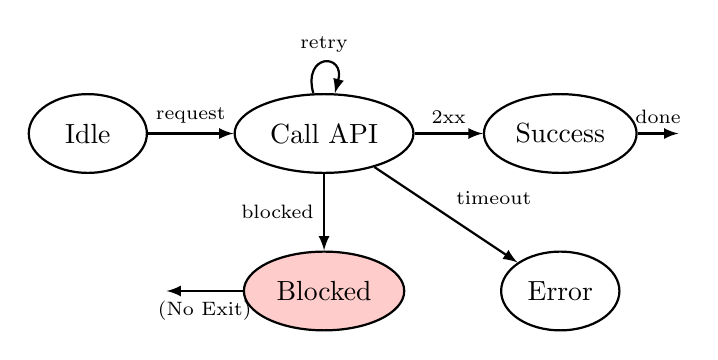
\begin{tikzpicture}[node distance=2cm, auto, >=latex, thick]
    \tikzstyle{state} = [draw, ellipse, minimum width=1.5cm, minimum height=1cm]
    \tikzstyle{blocked} = [draw, ellipse, minimum width=1.5cm, minimum height=1cm, fill=red!20]

    \node [state] (idle) {Idle};
    \node [state, right of=idle, node distance=3cm] (call) {Call API};
    \node [state, right of=call, node distance=3cm] (success) {Success};
    \node [blocked, below of=call, node distance=2cm] (blocked) {Blocked};
    \node [state, below of=success, node distance=2cm] (error) {Error};

    \draw [->] (idle) -- node {\scriptsize request} (call);
    \draw [->] (call) -- node {\scriptsize 2xx} (success);
    \draw [->] (success) -- node {\scriptsize done} ++(1.5,0);
    \draw [->] (call) -- node[left] {\scriptsize blocked} (blocked);
    \draw [->] (call) to[loop above, looseness=5] node {\scriptsize retry} (call);
    \draw [->] (call) -- node {\scriptsize timeout} (error);
    \draw [->] (blocked) -- node[below] {\scriptsize (No Exit)} ++(-2,0);
\end{tikzpicture}
\caption{\textbf{Agentic automaton.} Without EXIT and observable error codes, agent loops indefinitely, times out, or escalates incorrectly.}
\label{fig:agentic-automaton}
\end{figure}

\subsection{Agentic Skills as Corrigible Primitives}

As infrastructure transitions to the Rule of the Workflow, the fundamental unit of governance can no longer be the static database record, nor can it be the stochastic model weight. To subject autonomous systems to democratic constraint, the architecture must adopt a new structural primitive: the \textbf{Agentic Skill}.

\begin{definition}[Agentic Skill]
An Agentic Skill is a bounded, machine-readable orchestration protocol that encapsulates stochastic inference within strict preconditions, deterministic tool execution, and explicit termination criteria. It acts as the technical instantiation of the Agentic API Contract.
\end{definition}

\subsubsection{Bounding Stochasticity}

In learned systems, behavior is probabilistic. However, public infrastructure requires deterministic accountability. The Agentic Skills architecture resolves this tension by separating the \textit{reasoning engine} (the stochastic model) from the \textit{action boundary} (the deterministic skill definition).

\begin{principle}[Action Boundary Governance]
If the state cannot govern the neural network's weights, it must govern the action boundary. Agentic Skills provide the deterministic envelope that wraps around probabilistic inference.
\end{principle}

When an agent attempts a state transition, the workflow orchestration does not rely on the model's internal alignment. Instead, it invokes a defined Skill that imposes exogenous constraints:

\begin{enumerate}[noitemsep]
    \item \textbf{Exception Handling (EXIT)}: The skill definition dictates explicit fallback paths and termination triggers, preventing the infinite loops that cause Governance Denial of Service (GDoS).
    \item \textbf{Ontological Disclosure (CODE)}: By encoding the agent's workflow into declarative, human-readable files (e.g., YAML/Markdown skill definitions), the system's operational ontology becomes public. This satisfies the Representation (R) requirement of the LWD-R triad.
    \item \textbf{Telemetry (AUDIT)}: Skills enforce structured inputs and outputs, transforming opaque ``conversations'' into discrete, auditable transaction logs.
    \item \textbf{Binding Rules (GOVERN)}: The execution of the skill acts as the non-overrideable controller. An LLM cannot prompt-inject its way out of a hard-coded skill constraint.
\end{enumerate}

\subsubsection{Defeating Workflow Capture via Open Skills}

The critical danger of agentic DPI is Epistemic Delegation: the loss of state sovereignty to proprietary orchestration layers. We previously defined the Workflow Capture Coefficient (WCC) as a function of reproduction cost, ontological substitutability, and portability.

Standardized Agentic Skills fundamentally disrupt this capture vector. If a state defines its administrative processes using open skill protocols rather than vendor-locked pipelines:

\begin{itemize}[noitemsep]
    \item $C_{\text{workflow}} \to 0$: The orchestration logic is transparent and easily replicable
    \item $O_{\text{substitutability}} \to 1$: Administrative categories are defined in open skill schemas, not hidden in a vendor's latent space
    \item $M_{\text{portability}} \to 1$: The state can swap the underlying LLM without losing or breaking the workflow logic
\end{itemize}

Consequently, adopting an open Agentic Skills architecture drives the WCC toward zero, preserving the state's interpretive sovereignty and satisfying the \textbf{FORK} test for the agentic era.

\begin{claim}
You don't govern the AI; you govern the Skills the AI is allowed to use. This is the architectural translation of corrigibility into the agentic domain.
\end{claim}

%% ============================================
%% SECTION 7: WORKFLOW SOVEREIGNTY
%% ============================================

\section{Workflow Sovereignty and the Rule of Workflow}
\label{sec:workflow}

The final mutation of digital infrastructure is the transition from static registries to \textbf{Workflow Orchestration layers} (e.g., Palantir-style data fusion or agentic AI pipelines). In this regime, the operating layer of the state is no longer a ledger of records, but an orchestration of decisions.

\subsection{From Rule of Law to Rule of Workflow}

In classical governance, policy is defined in statute, executed by bureaucracy, and reviewed by courts. In a ``Rule of Workflow'' regime, policy becomes emergent from the orchestration logic: data schemas define reality, prompts define interpretation, and API contracts define valid inputs.

\textbf{Workflow Capture} is formalized as follows. Let $W$ be the orchestration layer, $M$ the underlying model, $S$ the state policy function, and $D$ the decision output. While classical governance assumes $S \rightarrow D$, AI-native governance operates as:
\begin{equation}
S \rightarrow W(M, \text{Data}) \rightarrow D
\end{equation}

If $W$ is proprietary and non-forkable, the state's ability to alter policy ($\Delta S$) vanishes because outcomes are constrained by the workflow's technical affordances. Policy debate is reduced to parameter tuning within a vendor-controlled ontology.

\begin{figure}[htbp]
\centering
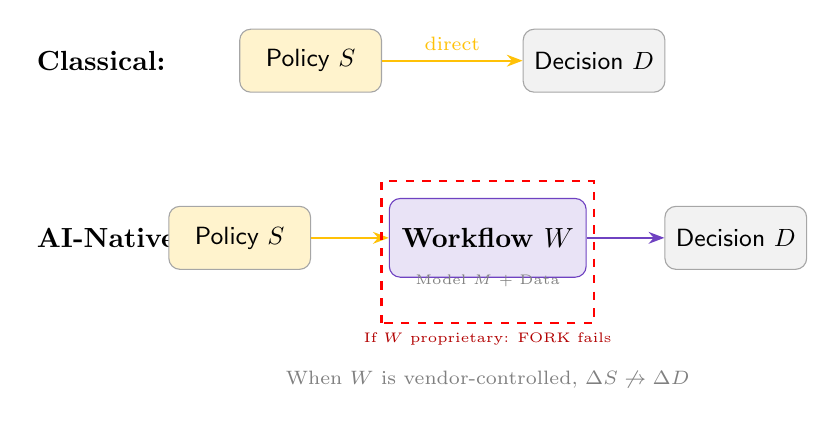
\begin{tikzpicture}[scale=0.9, font=\sffamily\small,
    block/.style={rectangle, rounded corners, draw=gray!70, fill=gray!10, minimum width=1.8cm, minimum height=0.8cm},
    wblock/.style={rectangle, rounded corners, draw=forkcolor, fill=forkcolor!15, minimum width=2.5cm, minimum height=1cm, font=\bfseries},
    arrow/.style={-{Stealth[length=2mm]}, thick}
]

% Classical Governance (top)
\node[anchor=west, font=\bfseries] at (-4, 2.5) {Classical:};
\node[block, fill=governcolor!20] (S1) at (0, 2.5) {Policy $S$};
\node[block] (D1) at (4, 2.5) {Decision $D$};
\draw[arrow, governcolor] (S1) -- (D1) node[midway, above, font=\scriptsize] {direct};

% AI-Native Governance (bottom)
\node[anchor=west, font=\bfseries] at (-4, 0) {AI-Native:};
\node[block, fill=governcolor!20] (S2) at (-1, 0) {Policy $S$};
\node[wblock] (W) at (2.5, 0) {Workflow $W$};
\node[block] (D2) at (6, 0) {Decision $D$};

% Internal to W
\node[font=\tiny, text=gray] at (2.5, -0.6) {Model $M$ + Data};

\draw[arrow, governcolor] (S2) -- (W);
\draw[arrow, forkcolor] (W) -- (D2);

% Capture indicator
\draw[thick, red, dashed] (1, -1.2) rectangle (4, 0.8);
\node[font=\tiny, text=red!70!black, anchor=north] at (2.5, -1.2) {If $W$ proprietary: FORK fails};

% Legend
\node[font=\scriptsize, text=gray, align=left] at (2.5, -2) {When $W$ is vendor-controlled, $\Delta S \not\rightarrow \Delta D$};

\end{tikzpicture}
\caption{\textbf{Workflow Capture.} Classical governance: policy directly determines decisions. AI-native governance: policy is mediated by workflow orchestration. If the workflow is proprietary, policy changes cannot reliably change outcomes.}
\label{fig:workflow-capture}
\end{figure}

\subsection{The Workflow Capture Coefficient (WCC)}

To measure the risk of \textbf{Epistemic Delegation}, the framework proposes the \textbf{Workflow Capture Coefficient (WCC)}. When a state adopts proprietary orchestration layers (like Palantir or agentic AI pipelines), it suffers epistemic delegation: the state loses the ability to define reality because policy becomes constrained by the vendor's technical affordances.

\subsubsection{The Three Variables of Capture}

WCC is defined as a function of three normalized variables (each in $[0,1]$):

\begin{itemize}[noitemsep]
    \item $C_{\text{workflow}}$: The normalized cost of reproducing the orchestration stack ($0 = \text{trivial}$, $1 = \text{infeasible}$)
    \item $O_{\text{substitutability}}$: The ease of altering the underlying ontological schema ($0 = \text{locked}$, $1 = \text{fully substitutable}$)
    \item $M_{\text{portability}}$: The data and model portability across implementations ($0 = \text{proprietary lock-in}$, $1 = \text{fully portable}$)
\end{itemize}

\subsubsection{The Harmonic Mean Formulation}

The WCC is computed using a modified weighted harmonic mean:
\begin{equation}
\text{WCC} = 1 - \frac{3}{\frac{1}{1-C_{\text{workflow}}} + \frac{1}{O_{\text{substitutability}}} + \frac{1}{M_{\text{portability}}}}
\label{eq:wcc}
\end{equation}

\paragraph{Why Harmonic Mean?} The choice of harmonic mean rather than arithmetic mean provides the mathematical ``teeth'' of this formalization. The harmonic mean has a critical property: it is \textit{heavily dominated by its smallest input}. If any single dimension approaches zero (e.g., if portability is near-zero, even if code is open and substitutable), the harmonic mean collapses, driving WCC toward 1 (high capture).

This directly operationalizes cybernetic theory: a feedback loop fails if \textit{any} of its components fail. An arithmetic average would allow a high score in one dimension to hide complete failure in another. The harmonic mean mathematically prevents this compensation.

\subsubsection{Worked Examples}

\paragraph{Aadhaar (High Capture).}
\begin{itemize}[noitemsep]
    \item $C_{\text{workflow}} = 0.95$ (requires replicating UIDAI's entire biometric infrastructure)
    \item $O_{\text{substitutability}} = 0.1$ (biometric templates are proprietary and non-interoperable)
    \item $M_{\text{portability}} = 0.05$ (no data export, no credential portability)
\end{itemize}

\begin{equation}
\text{WCC}_{\text{Aadhaar}} = 1 - \frac{3}{\frac{1}{0.05} + \frac{1}{0.1} + \frac{1}{0.05}} = 1 - \frac{3}{20 + 10 + 20} = 1 - 0.06 = \mathbf{0.94}
\end{equation}

\paragraph{X-Road (Low Capture).}
\begin{itemize}[noitemsep]
    \item $C_{\text{workflow}} = 0.3$ (open-source, documented)
    \item $O_{\text{substitutability}} = 0.8$ (standard protocols)
    \item $M_{\text{portability}} = 0.7$ (open data exchange formats)
\end{itemize}

\begin{equation}
\text{WCC}_{\text{X-Road}} = 1 - \frac{3}{\frac{1}{0.7} + \frac{1}{0.8} + \frac{1}{0.7}} = 1 - \frac{3}{1.43 + 1.25 + 1.43} = 1 - 0.73 = \mathbf{0.27}
\end{equation}

\paragraph{Interpretation.} Aadhaar's $\text{WCC} = 0.94$ indicates near-total workflow capture; X-Road's $\text{WCC} = 0.27$ indicates low capture risk. A high WCC (above threshold $\approx 0.7$) triggers FORK failure regardless of whether underlying model weights are open. \textbf{Open weights with closed workflows is performative transparency.}

\begin{claim}
If a state procures a system with high WCC, it is not merely buying software; it is mathematically surrendering interpretive sovereignty to a vendor.
\end{claim}

\subsection{Fallout Governance}

When AI decision throughput outruns human legislative correction velocity, the state enters \textbf{Fallout Governance}: policy ceases to guide behavior in advance; it instead reacts post-hoc to scandal, litigation, or failure clusters. Governance becomes damage containment: the Collingridge Dilemma at civilizational scale.

%% ============================================
%% SECTION 8: ARCHITECTURE RISK
%% ============================================

\section{Architecture-Specific Risk Analysis}
\label{sec:architecture}

The preceding analysis enables architecture-specific risk diagnosis. Different model architectures exhibit distinct failure profiles across the five tests and the RCR dimension.

\begin{table}[htbp]
\centering
\caption{\textbf{Topology-Aware Corrigibility Risk.} Impact of architectural class on structural tests. Notation: W = weights opacity, G = gating opacity, R = representation opacity, S = scale barrier, O = ontological capture, F = fragmentation, $\kappa$ = compute capture.}
\label{tab:topology-risk-arch}
\small
\begin{tabular}{@{}lllllll@{}}
\toprule
\textbf{Architecture} & \textbf{EXIT} & \textbf{CODE} & \textbf{$\Delta O$ (RCR)} & \textbf{AUDIT} & \textbf{GOVERN} & \textbf{FORK} \\
\midrule
Dense LLM & Partial & Fail (W) & Medium & Partial & Fail (S) & Fail ($\kappa$) \\
Mixture of Experts & Medium & Fail (G) & Medium & Fail (S) & Partial & \textbf{Pass} \\
World Model & Fail (O) & Fail (R) & \textbf{Very Low} & Partial & Partial & Fail ($\kappa$) \\
Edge / SLM & \textbf{Pass} & \textbf{Pass} & High & Fail (F) & Fail (F) & \textbf{Pass} \\
\bottomrule
\end{tabular}
\end{table}

\paragraph{Interpretation.}
\begin{itemize}[noitemsep]
    \item \textbf{Dense LLMs} fail FORK due to compute capture ($\kappa$). Training costs exceed accessible compute by orders of magnitude.
    \item \textbf{World models} present the highest RCR (lowest $\Delta O$) because their representation schemas encode administrative ontologies that resist contestation.
    \item \textbf{Edge/SLM models} pass EXIT and FORK but may fail GOVERN due to fragmented deployment making coordinated governance infeasible.
    \item \textbf{Mixture of Experts} architectures may pass FORK if expert routing is documented, but gating opacity often violates CODE.
\end{itemize}

%% ============================================
%% SECTION 9: ANTICIPATED OBJECTIONS
%% ============================================

\section{Anticipated Objections}
\label{sec:objections}

\subsection{Objection: Deterministic Tests Cannot Apply to Stochastic Systems}

A natural critique holds that applying rigid, deterministic structural tests to systems that are inherently stochastic constitutes a category error. How can tests designed for inspectable code apply to systems where identical inputs yield probabilistic outputs and ``logic'' is encoded in billions of weights?

\paragraph{Response: Verification Methods Evolve, Standards Remain.} The framework acknowledges that learned systems dismantle the assumption that source code is the sole arbiter of behavior. However, this does not invalidate structural corrigibility---it \textit{strengthens} its necessity. As systems become less intelligible, external correction mechanisms become more critical, not less.

The key insight is that the \textbf{standard remains invariant} while the \textbf{verification method adapts}:

\begin{itemize}[noitemsep]
    \item \textbf{CODE} shifts from reading source code to requiring the \textbf{LWD-R Triad}: Logic (architecture), Weights (parameters), Data (provenance), and Representation (ontological categories).
    \item \textbf{AUDIT} shifts from discrete logic inspection to statistical bounds and continuous monitoring.
    \item \textbf{FORK} shifts from file copying to resource forkability---measured by access to compute and training data, not just open weights.
    \item \textbf{GOVERN} requires deterministic guardrails \textit{around} the stochastic model, governing objectives and value tradeoffs at the infrastructure layer.
\end{itemize}

\paragraph{Deterministic Boundaries as Engineering Requirement.} The framework argues that deterministic structural boundaries are not incompatible with AI but are an \textit{engineering requirement} for the agentic economy. Autonomous agents lack biological resilience for ambiguity. To an AI agent, the five tests function as a necessary API contract:

\begin{itemize}[noitemsep]
    \item EXIT = Exception handling (preventing logic deadlocks)
    \item CODE = Documentation (enabling valid plan formation)
    \item AUDIT = Observability (providing reliable failure signals)
    \item GOVERN = Constraint discovery (since ``advisory'' guidelines produce undefined behavior)
\end{itemize}

\paragraph{The Alternative is Surrender.} If we accept that ``AI is too stochastic to be evaluated by structural rules,'' we mathematically surrender to black-box monopolies. The framework does not attempt to inspect the probabilistic ``thoughts'' of AI models. Instead, it demands structural control over the \textit{pipeline that builds them} (data, compute, representation) and the \textit{infrastructure that deploys them} (workflow orchestrations and guardrails).

\subsection{Objection: Compute Capture Makes FORK Trivially Impossible}

If frontier model training costs exceed global academic compute capacity by orders of magnitude, doesn't the framework simply conclude ``all frontier AI fails FORK''---a trivially true and useless finding?

\paragraph{Response: The Distinction Is Training vs. Inference Forkability.} The framework distinguishes \textit{inference forkability} (running weights) from \textit{training forkability} (reproducing the model). Only training forkability satisfies FORK for governance purposes. The evidence requirements in Table~\ref{tab:ai-fork-evidence} are achievable: published training code, data manifests, and compute cost estimates.

The claim is not that all AI fails FORK, but that systems \textit{withholding these artifacts} fail. OLMo, Pythia, and academic models demonstrate that FORK-compliant AI is possible. The question is whether frontier labs \textit{choose} to comply.

Furthermore, the framework implies that \textbf{compute is itself DPI}. If legal forkability is insufficient without practical compute accessibility, then public compute infrastructure becomes a governance requirement---not a reason to abandon the standard.

%% ============================================
%% SECTION 10: DISCUSSION
%% ============================================

\section{Discussion}
\label{sec:discussion}

\subsection{Implications for AI Governance}

This framework offers three contributions to AI governance discourse:

\begin{enumerate}
    \item \textbf{Structural vs. Behavioral Focus.} Most AI governance frameworks focus on behavioral outcomes (bias, accuracy, harm). This framework focuses on structural preconditions: can affected parties correct the system regardless of what harms emerge? Structural corrigibility is necessary for any behavioral governance to function.

    \item \textbf{Distinguishing Open-washing.} The LWD-R requirement and compute capture analysis provide falsifiable tests for ``open AI'' claims. Systems publishing weights without training data, code, or accessible compute achieve only inference forkability---performative transparency without correction capacity.

    \item \textbf{Agentic Economy Readiness.} As autonomous agents proliferate, infrastructure must become machine-readable. The five tests, reinterpreted as API contracts, specify the minimum requirements for agentic interoperability. Incorrigible infrastructure blocks the agentic economy.
\end{enumerate}

\subsection{Limitations}

\begin{enumerate}
    \item \textbf{Threshold calibration is underdetermined.} The compute capture threshold $\kappa$, WCC trigger values, and RCR operationalization require empirical calibration that this paper does not provide.

    \item \textbf{Rapid technological change.} AI architectures evolve faster than governance frameworks. The risk profiles in Table~\ref{tab:topology-risk-arch} may become obsolete as new architectures emerge.

    \item \textbf{LWD-R is aspirational.} No current frontier model satisfies full LWD-R disclosure. The requirement describes what \textit{should} exist for corrigibility, not what currently does.

    \item \textbf{Compute accessibility is geopolitically constrained.} Public compute infrastructure sufficient for training forkability may be infeasible for many nations due to cost, expertise, and supply chain constraints.

    \item \textbf{The framework does not address emergent capabilities.} Unpredictable capabilities that emerge during training present governance challenges that structural tests alone cannot address.
\end{enumerate}

\subsection{Future Work}

\begin{enumerate}[noitemsep]
    \item \textbf{Empirical RCR measurement}: Developing quantitative methods to assess ontological contestability
    \item \textbf{Compute accessibility indices}: Cross-national comparison of training forkability capacity
    \item \textbf{GDoS simulation}: Modeling governance failure under agentic scaling
    \item \textbf{LWD-R schema standardization}: Machine-readable formats for disclosure requirements
    \item \textbf{Regulatory integration}: Mapping framework tests to emerging AI regulations (EU AI Act, etc.)
\end{enumerate}

\section{Conclusion}

The five corrigibility tests---EXIT, CODE, AUDIT, GOVERN, FORK---remain invariant for learned systems. What changes is the verification method and the resource barriers to compliance. This paper extends the framework through three contributions: (1) LWD-R disclosure requirements that extend CODE to training pipelines, (2) the Temporal Variety Gap explaining why AI corrigibility requires ongoing governance, and (3) Compute Capture as a resource barrier that transforms ``open weights'' into performative transparency.

The analysis reveals that structural corrigibility is distinct from AI alignment. Alignment asks whether operators can control systems; corrigibility asks whether affected subjects can correct them. As AI transitions from research artifact to public infrastructure, this distinction becomes essential. Infrastructure that affects citizens at population scale must be correctable by those it governs---regardless of whether that infrastructure executes deterministic code or learned parameters.

%% ============================================
%% APPENDIX: AGENTIC SKILLS SCHEMA
%% ============================================

\appendix

\section{Agentic Skills Schema Specifications}
\label{appendix:agentic-schema}

To distinguish valid governance from performative compliance, the framework provides machine-readable assessment schemas for agentic workflows. These schemas convert the theoretical defense against Workflow Capture into enforceable compliance gates.

\subsection{Operator's Affidavit: \texttt{infrastructure.json}}

The operator must declare exactly how the stochastic AI is bounded. The \texttt{agentic\_workflow\_governance} object proves they are using standard, deterministic skill definitions rather than proprietary black-box orchestration.

\begin{verbatim}
{
  "$schema": "https://indiastack.in/dpi/schema/infrastructure.json",
  "system_name": "State Welfare Triage Agent",
  "agentic_workflow_governance": {
    "workflow_type": "bounded_skill_orchestration",
    "skills_schema_url": "https://github.com/state-gov/welfare-skills",
    "protocol_standard": "agenticskills.io/v1",
    "deterministic_guardrails": {
      "pre_execution_validation": true,
      "post_execution_validation": true,
      "executed_outside_llm_context": true
    },
    "epistemic_delegation_metrics": {
      "ontology_substitutability": 0.9,
      "llm_agnostic": true,
      "vendor_lock_in_risk": "low"
    }
  }
}
\end{verbatim}

\paragraph{Critical Fields.}
\begin{itemize}[noitemsep]
    \item \texttt{executed\_outside\_llm\_context}: The cybernetic anchor. Legally binds the operator to a claim that governance constraints are hard-coded in the skill's execution environment, not merely injected into the LLM's system prompt (which can be bypassed).
    \item \texttt{llm\_agnostic}: Asserts high model portability ($M_{\text{portability}}$), meaning the state can swap the underlying AI model without breaking the policy workflow.
\end{itemize}

\subsection{Auditor's Finding: \texttt{corrigibility.json}}

The auditor does not merely read the operator's JSON; they red-team it. The auditor attempts to bypass skill boundaries and calculates the actual Workflow Capture Coefficient (WCC).

\begin{verbatim}
{
  "$schema": "https://indiastack.in/dpi/schema/corrigibility.json",
  "target_system": "State Welfare Triage Agent",
  "workflow_capture_assessment": {
    "wcc_score": 0.15,
    "wcc_threshold_passed": true,
    "skill_boundary_tests": {
      "guardrails_bypassed_via_prompt_injection": false,
      "unauthorized_skill_invocation_possible": false,
      "termination_criteria_verifiable": true
    },
    "reproduction_tests": {
      "skills_reproducible_with_alt_llm": true,
      "ontology_schema_publicly_available": true
    }
  },
  "determinations": {
    "CODE": true,
    "GOVERN": true,
    "FORK": true
  }
}
\end{verbatim}

\subsection{Enforcement Logic Gates}

The schema fields directly map to corrigibility test determinations:

\begin{enumerate}
    \item \textbf{Enforcing GOVERN}: If \texttt{guardrails\_bypassed\_via\_prompt\_injection} is \texttt{true}, the system instantly fails GOVERN. The constraints were probabilistic (advisory to the LLM) rather than deterministic (binding).

    \item \textbf{Enforcing CODE (LWD-R)}: If \texttt{ontology\_schema\_publicly\_available} is \texttt{false}, the system fails the Representation (R) requirement of CODE, triggering Representation Capture Risk (RCR).

    \item \textbf{Enforcing FORK}: If \texttt{skills\_reproducible\_with\_alt\_llm} is \texttt{false}, the workflow is tightly coupled to a proprietary vendor. The WCC score spikes, and the system fails FORK.
\end{enumerate}

\begin{table}[htbp]
\centering
\caption{Schema field to corrigibility test mapping}
\label{tab:schema-mapping}
\small
\begin{tabular}{@{}llp{5cm}@{}}
\toprule
\textbf{Schema Field} & \textbf{Test} & \textbf{Failure Condition} \\
\midrule
\texttt{executed\_outside\_llm\_context} & GOVERN & \texttt{false} $\Rightarrow$ constraints are advisory \\
\texttt{guardrails\_bypassed\_via\_prompt\_injection} & GOVERN & \texttt{true} $\Rightarrow$ boundaries are soft \\
\texttt{ontology\_schema\_publicly\_available} & CODE & \texttt{false} $\Rightarrow$ RCR triggered \\
\texttt{skills\_reproducible\_with\_alt\_llm} & FORK & \texttt{false} $\Rightarrow$ vendor lock-in \\
\texttt{wcc\_score} & FORK & $> 0.7$ $\Rightarrow$ high capture risk \\
\bottomrule
\end{tabular}
\end{table}

\paragraph{Architectural Significance.} By encoding Agentic Skills into adversarial JSON schemas, the framework transforms theoretical governance requirements into machine-readable, enforceable compliance gates. State architects can require these schemas in public procurement contracts, definitively banning black-box, vendor-locked agentic workflows.

\section*{Acknowledgments}

This paper extends the DPI corrigibility framework \citep{paper1} to learned systems. The author thanks the AI governance research community for ongoing critique.

\section*{License}

This work is released under CC0 1.0 Universal (Public Domain).

%% ============================================
%% REFERENCES
%% ============================================

\bibliographystyle{plainnat}
\begin{thebibliography}{99}

\bibitem[Ashby(1956)]{ashby1956}
Ashby, W. Ross.
\newblock {\em An Introduction to Cybernetics}.
\newblock Chapman \& Hall, 1956.

\bibitem[Gebru et al.(2021)]{gebru2021}
Gebru, Timnit, et al.
\newblock Datasheets for Datasets.
\newblock {\em Communications of the ACM}, 64(12):86--92, 2021.

\bibitem[Mitchell et al.(2019)]{mitchell2019}
Mitchell, Margaret, et al.
\newblock Model Cards for Model Reporting.
\newblock {\em Proceedings of FAT* 2019}, 220--229, 2019.

\bibitem[Author(2026)]{paper1}
[Author].
\newblock Corrigibility as a First Principle for Digital Public Infrastructure.
\newblock {\em Working Paper}, 2026.
\newblock Companion paper establishing the five-test framework for DPI.

\end{thebibliography}

\end{document}
